%auto-ignore
%      this ensures the arxiv doesn't try to start TeXing here.
%!TEX root = super_lattice_models_draft.tex
%      prev line helps TeXShop do the right thing



%%%%%%%%%%%%%%%%%% 
\section{Discussion} \label{discussion}
%%%%%%%%%%%%%%%%%%
\davex{I think generally the discussion is nice. 
But we can probably trim it by quite a bit. 
There are a few main points that we could highlight and then remove most of the details.
Do you guys think we should keep these for our friends?}

\davex{I think we should condense this paragraph (possibly remove).
And lets also remove the figure.}
One exciting aspect of the fermionic topological orders we have studied in this paper is their potential quantum information 
applications, which we now briefly speculate on. 
First, we can consider a hybrid system with spin structure defects and deconfined anyonic excitations.
Consider the scenario where several q-type defects terminate at a boundary of a sample, as shown in Fig.\ref{QCApplication}, where the q-type defects are drawn as orange lines.
\davex{spin structure defects hosting q-type particles.
The following is probably too much detail. 
Roughly: `the q-type vortices naturally provide clifford gates, while the deconfined anyonic excitations supplement this gate set with the usual TQC'}
For a system with $n$ such defects,  
the computational space associated with the defects $Q_1,Q_2,\dots,Q_n$ is the fusion space $V^{Q_1 Q_2 \cdots Q_n}$. 
There are two kinds of logical operations we can perform on the defects:
one is given by braiding the deconfined anyons in the bulk, and is familiar from conventional topological quantum computation.
The other is given by the action of $\End(Q_1)\tp\End(Q_2)\tp\dots\tp\End(Q_n)\cong\cliff_1^{\tp n} \cong \cliff_n$ on the defects.
\davex{The following sentence we should keep, but also reference the appropriate paper and say a little more carefully what `nearly universal' means. 
I'll dig up the paper shortly.}
It is known that the resulting clifford gates are nearly universal, meaning that the addition of a single entangling gate results in a universal gate set.
\davex{I think the following is true but not necessary to keep.}
The action of $\cliff_n$ can be implemented by connecting Kitaev wires to the terminations of the q-type defects, as shown in Fig.~\ref{QCApplication}, and tuning the flux through those wires. 
Adiabatically tuning the flux by one flux quantum, one ejects a pair of electrons into the q-type defects, and hence applies the Clifford gate $\Gamma_i \tp \Gamma_j$, where $\Gamma_i$ is the odd generator 
of the $i$th tensor factor in $\cliff^{\tp n}$.
%\dave{I'll make this more precise if we want to include a discussion of this sort.
%It may make our paper more appealing to some people.}
%\ethan{should try to make this better}

\begin{figure}
\begin{center}
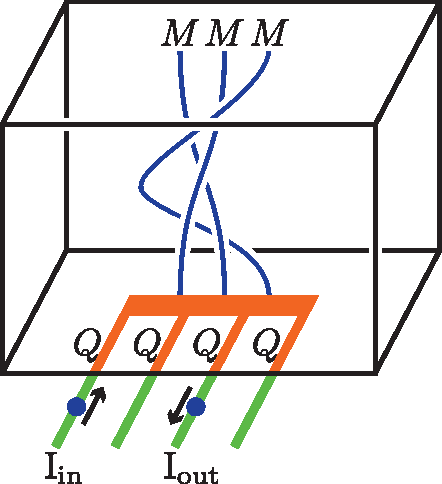
\includegraphics[scale=.8]{QCApplication.pdf}
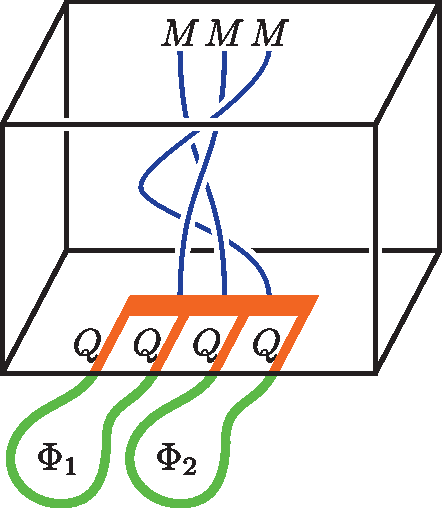
\includegraphics[scale=.8]{QCApplication2.pdf}
\caption{\label{QCApplication}  
An illustration of one possible quantum information application of the topological orders discussed in the main text. 
In this setup, we have four q-type defects $Q$ (orange lines) which terminate at the boundary of the sample, and are strongly hybridized with two Kitaev wires (green lines). 
By adiabatically tuning the flux $\Phi_j$ through the Kitaev wires, one implements Clifford gates acting
on the Clifford algebra $\cliff_4$. 
In addition to the Clifford gates, we can also braid the deconfined m-type particles appearing the fusion space of the q-type defects (blue lines) to realize a richer gate set. 
}
\end{center}
\end{figure}

\davex{Also need to think about this sentence. 
Ethan, maybe we should Skype about it. 
Is the main purpose to mention the connection between $p+ip$ SC and the way we treat physical fermions? \ethan{yes. We were always wondering how to show the existence of a p+ip SC in the background, and this paragraph is mentioning that}
I think this has to be (atleast in part) in the literature already. 
E.g., the mathy people who clossified topological insulators (I'm not super familiar with the literature there but presumably that's a good place to look) .}
Additionally, it would be useful to make more precise connections between physical entities and some of the mathematical 
devices we have used to construct the fermionic theories 
we have studied. 
In particular, it would be useful to clarify the precise physical meaning of the complex line bundle 
and the ``back wall'' that we use to perform fermion condensation. 
In simple examples like the $C_2$ theory, the most natural interpretation for these constructs 
seems to be that they constitute a topological p-wave superconductor.
Indeed, the way we treat the physical fermions we use to perform condensation 
in our models is identical to the behavior of 
superconductors: they are 
free fermion states, 
%\kw{``states of states"?}
where wavefunctions that differ by pairs of 
fermions are related by a phase. 
The specialization to the p-wave pairing channel is made because of the spinless-ness
of the fermions we use to induce the condensation, which we assumed from the very 
beginning.  
The superconducting nature of the devices we use to perform condensation is forced on us
by our assumption that the emergent fermion $\psi$ we condense possesses $\zt$
fusion rules, and that in the complex line bundle we construct, pairs of
$\psi$ worldline endpoints can be created or destroyed in pairs. 
Evidence for the presence of a p-wave superconductor is most clearly seen in the $C_2$ theory, 
where additional corroboration emerges after we construct $\tube(C_2)$: 
restricting to the non-bounding $NN$ spin sector, both the modular $S$ and $T$ matrices 
factorize as $S=S_{Ising}\tp S_{p\pm ip}, T = T_{Ising} \tp T_{p\pm ip}$ (where the 
choice of $\pm$ is determined by the ``angular momentum'' of the fermionic dots 
in our graphical calculus, i.e. the choice of $\pm A^4$ when removing a semicircular fermion
worldline), suggesting a possible interpretation of this sector 
as a stack of the origin Ising theory with a topological superconductor. 
Indeed, this was noticed recently in \cite{ware2016}.
Furthermore, that the parity of the ground states on the torus with $(N,N)$ spin structure is always 
odd agrees with this interpretation, since the fermion parity of a topological 
p-wave superconductor on such a torus is always odd \cite{you2015}.
For more
complicated theories like the $\halfesix/y$ theory, whose modular matrices do not obviously contain a superconductor-related factor, 
it is at present unclear how precise this interpretation really is. 

\davex{I think this paragraph is a little outdated, we don't do braiding anymore.}
\ethan{This paragraph was written {\it because} we don't do braiding anymore!}
In our discussion of the modular $S$ and $T$ matrices in each of the examples we've worked out, 
we have focused on the modular transformation perspective, rather than on the braiding statistics perspective. 
For example, we have computed the $S$-matrix by considering the way it acts to exchange the two 
cycles of the torus and 
we have not focused on the statistical picture behind the $S$-matrix, in which matrix elements $S_{ab}$ correspond to double braids between $a$ and $b$ particles. 
While we have checked that the computation of double braids reproduces the correct $S$-matrix 
in the tube algebra of the $C_2$ theory, some subtleties involving relative spin structures rear their heads when trying to compute particular braiding data in more general settings. 
We plan to address these subtleties in future work. 

We have analyzed fermion condensation in all its different guises, but have had little to say about the reverse procedure:
starting from a fermionic phase and ``bosonizing'' to obtain a bosonic one. Roughly, this can be done by 
``summing over spin structures'' (see e.g. \cite{bhardwaj2016,kapustin2017}).
Since bosonic theories are defined without reference to spin structures, to obtain a bosonic theory from a fermionic 
one in which $\psi$ has been condensed, we must remove the spin structure dependence. 
Schematically, we can consider ``averaging'' over spin structures by condensing spin structure defect lines: since $\psi$ endpoints braid nontrivially with the defect lines the resulting low-energy theory contains no 
$\psi$ endpoints, and $\psi$ ceases to be isomorphic to the vacuum. 
This process is related to the modular extension construction discussed in \cite{Lan2016b}: a fermionic theory $\mcc /\psi$ with $\psi$ considered as a distinct object is not modular, but can be made modular
constructing a modular extension of $\mcc / \psi$. The minimal such extensions reproduce the different possible 
parent theories $\mcc$. 

A natural question to ask at this stage is: what kind of fermionic topologically ordered phases can exist? 
At this point, there seem to be essentially two broad classes of fermionic phases, both of which can be obtained from bosonic theories. 
The first class is ``trivially'' fermionic: suppose we have some bosonic theory $\mcc$. 
We may then obtain a fermionic theory by simply stacking $\mcc$ with a phase of physical fermions $\mcc_{f} = \mcc \boxtimes {\rm sVec}$, where sVec is the category of supervector spaces, whose simple objects are ${\rm sObj}({\rm sVec}) = \{\unit,f\}$, with $f$ a physical fermion. 
$\mcc_f$ is fermionic, but in a rather trivial sense, since its ``fermionic-ness'' factors and is contained entirely within the sVec part of the product. 
The other (more interesting) way to obtain a fermion phase is to perform fermion condensation, which as we have 
mentioned amounts to stacking $\mcc$ with a phase of physical fermions and condensing pairs of emergent and physical fermions. 
This yields $\mcc_f' = (\mcc \boxtimes {\rm sVec}) / (\psi \boxtimes f),$
where $\psi \in \mcc$ is an emergent fermion. 
It is then natural to wonder whether all fermionic topological phases can be obtained by stacking or condensation in this way. 
It seems reasonable to bet that they can -- given a fermionic phase, one can always perform bosonization 
to obtain a bosonic phase, which will contain a fermion that can be condensed to reproduce the 
original fermionic theory. 
\kw{Doesn't the Usher paper address this?}
\ethan{sorta, not convinced that he does this correctly. Kapustin does a better job I think, but even 
there I don't think he does things in full generality}
\davex{I think the question `it is natural to wonder whether all SPC's can arise from fermion condensation' should be the main focus of the paragraph}

%\ethan{talk about $\mcc \boxtimes ({\rm sVec})^{\boxtimes n}$ as adding on a bunch of superconductors, and chiral charge stuff ($c_-$ for invertible fermionic orders is quantized as $n/2$ from cobordism argument)} 
%\ethan{mention difference between our approach and ``double the objects'' approach of wen in 1507.04673}
%\ethan{inverse of condensation is modular extension, and there are 16 modular extensions of sVec: eight Ising ones and eight TC-like ones (arXiv:0906.0620)}

On the more formal side, it would be interesting to extend our methods to theories where particles other than fermions are condensed. 
The simplest possible generalization would be to consider the condensation of objects which obey $\zz_r$ (with $r>2$) 
\kw{I changed $n>2$ to $r>2$; correct?}
\ethan{yes}
fusion rules. 
Instead of spin structures, condensing such objects would require equipping the manifold on which the theory is defined with an $r$-spin structure, 
which could have interesting consequences for the structure of the 
tube algebra. \ethan{Kevin, are you planning on thinking about this more?} 
\kw{Yes, planning, but so far no significant doing.}
Additionally, in our use of spin structures %(technically a pin$^+$ structure, see Appendix \ref{pins_and_reflection}) 
to perform fermion condensation, we have tacitly assumed that the physical fermions which provide the spin structure are {\it uncharged}. 
If the physical realization we have in mind for these fermions carries a $U(1)$ charge (in scenarios where 
the physical fermions are not provided by superconductors), we would need to generalize this to a spin$_c$ structure instead. 
Whether or not these modifications would have any qualitative effects on the structure of the resulting condensed theories 
is presently unclear.  

\davex{Could say that we (essentially) get gapped boundaries to bosonic TO's for free, but did not discuss this.}

 
 \paragraph{Acknowledgements}
Ethan Lake and Dave Aasen are grateful to Ryan Thorngren and \dots for discussions. Dave Aasen gratefully acknowledges support from the KITP Graduate Fellows Program, the National Science Foundation through grant DMR- 1723367
and the Caltech Institute for Quantum Information and Matter, 
an NSF Physics Frontiers Center with support of the Gordon and Betty Moore Foundation through Grant GBMF1250.
Ethan Lake is supported by the Fannie and John Hertz Foundation.
Dave Aasen and Ethan Lake acknowledge support by the 2016 Boulder Summer School for Condensed
Matter and Materials Physics through NSF grant DMR-13001648.
Kevin Walker thanks Zhenghan Wang and Scott Morrison for helpful conversations, and
thanks the Aspen Center for Physics and  the Mathematisches Forschungsinstitut Oberwolfach
for providing stimulating research environments.

